\documentclass[a4paper]{article}
% \documentclass{book}
\usepackage[utf8]{inputenc}
\usepackage[T2A]{fontenc}
\usepackage[english, russian]{babel}
\usepackage[left=25mm, top=20mm, right=25mm, bottom=30mm, nohead, nofoot]{geometry}
\usepackage{amsmath, amsfonts, amssymb} % математический пакет
\usepackage {fancybox, fancyhdr}
\pagestyle{fancy}
\fancyhf{}
\fancyhead[R]{Винер Даниил. БЭАД232}
\fancyfoot [R] {\thepage}
\fancyhead[L]{Математический анализ. Коллоквиум—3}
\setcounter {page}{1}
\headsep=10mm
\usepackage{xcolor}
\usepackage{blindtext}
\usepackage[T1]{fontenc}
\usepackage {hyperref}
\hypersetup{colorlinks=true, allcolors= [RGB]{010 090 200}} % цвет ссылок
\usepackage {setspace}
\usepackage[pdftex]{graphicx}
\usepackage{ dsfont }
\usepackage{array}
\setcounter{MaxMatrixCols}{20}
\usepackage{enumerate}
\usepackage{listings}
\usepackage{color}
\definecolor{dkgreen}{rgb}{0,0.6,0}
\definecolor{gray}{rgb}{0.5,0.5,0.5}
\definecolor{mauve}{rgb}{0.58,0,0.82}
\lstset{frame=tb,
  language=Python,
  aboveskip=3mm,
  belowskip=3mm,
  showstringspaces=false,
  columns=flexible,
  basicstyle={\small\ttfamily},
  numbers=none,
  numberstyle=\tiny\color{gray},
  keywordstyle=\color{blue},
  commentstyle=\color{dkgreen},
  stringstyle=\color{mauve},
  breaklines=true,
  breakatwhitespace=true,
  tabsize=3
}
\usepackage{tabularx}
\usepackage{multirow}
\usepackage{ upgreek }
\usepackage{tikz}
\usepackage{indentfirst}
\usepackage{hyperref}
\usepackage{mathrsfs}

\usepackage[utf8]{inputenc}
\usepackage{tcolorbox}

\newtcbox{\mybox}{colback=white,boxrule=0.5pt}

\newcommand{\mysection}[1]{
    \begin{tcolorbox}
        \subsection{#1}
    \end{tcolorbox}
}
\makeatletter
\newcommand\binomialCoefficient[2]{%
    % Store values 
    \c@pgf@counta=#1% n
    \c@pgf@countb=#2% k
    %
    % Take advantage of symmetry if k > n - k
    \c@pgf@countc=\c@pgf@counta%
    \advance\c@pgf@countc by-\c@pgf@countb%
    \ifnum\c@pgf@countb>\c@pgf@countc%
        \c@pgf@countb=\c@pgf@countc%
    \fi%
    %
    % Recursively compute the coefficients
    \c@pgf@countc=1% will hold the result
    \c@pgf@countd=0% counter
    \pgfmathloop% c -> c*(n-i)/(i+1) for i=0,...,k-1
        \ifnum\c@pgf@countd<\c@pgf@countb%
        \multiply\c@pgf@countc by\c@pgf@counta%
        \advance\c@pgf@counta by-1%
        \advance\c@pgf@countd by1%
        \divide\c@pgf@countc by\c@pgf@countd%
    \repeatpgfmathloop%
    \the\c@pgf@countc%
}
\makeatother


\newcommand{\qed}{\hfill$\square$}
\newcommand{\m}[1]{\mathbf{#1}}

\begin{document}
\tableofcontents
\newpage
\section{Вопросы}
\subsection{Что такое высшие дифференциалы отображения $F:\mathbb{R}^{n}\to\mathbb{R}^{m}$}
Рассмотрим дифференцируемое отображение $F:\mathbb{R}^n \to \mathbb{R}^m$ в каком-то открытом $\mathscr{U} \subseteq \mathbb{R}^n$, 
т.е. для каждой точки $\mathbf{p} \in \mathscr{U}$ у нас есть линейное отображение $(\mathrm{d}F)_{\mathbf{p}}: \mathbb{R}^n\to \mathbb{R}^m$

Так как линейные отображения из $\mathbb{R}^n$ в $\mathbb{R}^m$ — это просто матрицы размера $n\times m$, то дифференцируемость отображения $F$ в $\mathscr{U}$ означает, что у нас есть отображение
$$
\mathrm{d}F: \mathscr{U} \to \mathrm{Mat}_{n\times m}(\mathbb{R}), \qquad \mathbf{p} \mapsto (\mathrm{d}F)_{\mathbf{p}}.
$$

С другой стороны, пространство матриц $\mathrm{Mat}_{n\times m}(\mathbb{R})$ — векторное пространство, которое можно отождествить (=изоморфно) с $\mathbb{R}^{nm}$

Тогда мы можем поставить вопрос о дифференцируемости отображения $\mathrm{d}F$ и получить отображение
$$
\mathrm{d}^2(F): = \mathrm{d}(\mathrm{d}F): \mathscr{U}' \to \mathrm{Mat}_{n \times nm}(\mathbb{R}),
$$
где $\mathscr{U}'$ открыто в $\mathscr{U}$

Таким образом, мы получаем отображения (если они существуют)
$$
F:=\mathrm{d}^0F,\quad  \mathrm{d}F,\quad \mathrm{d}^2(F): = \mathrm{d}(\mathrm{d}F), \ldots, 
$$
среди которых $\mathrm{d}^k(F)$ при $k>1$ называются \textbf{высшими дифференциалами}

\subsection{Пусть дана $m$-раз дифференцируемая функция $f:\mathbb{R}^{n}\to\mathbb{R}$, то как выглядит общая формула для дифференциала $(\mathrm{d}^kf)$}

% Имеем $n$-раз дифференцируемую функцию $f:\mathbb{R}^n \to \mathbb{R}$ в окрестности $\mathscr{U}$ точки $\m{a}$. Мы знаем, что
% $$
% (\mathrm{d}f)_\m{a}(\m{h}) = \begin{pmatrix}
% f'_{x_1}(\m{a}) & \ldots & f'_{x_n}(\m{a})
% \end{pmatrix} \begin{pmatrix}
% h_1 \\ \vdots \\ h_n
% \end{pmatrix} = f_{x_1}'(\m{a})h_1 + \cdots + f_{x_n}'(\m{a})h_n
% $$

% Найдём $(\mathrm{d}^n(f))_\m{a}(\m{h}): = \mathrm{d}(\mathrm{d}^{n-1}f)_\m{a}(\m{h})$

% Пусть $C^\infty(\mathbb{R}^n)$ есть множество гладких (=бесконечно дифференцируемых) дифференцируемых функций $f:\mathbb{R}^n \to \mathbb{R}$. Рассмотрим следующие отображения:
% $$
% \frac{\partial}{\partial x_i}: C^\infty(\mathbb{R}^n) \to C^\infty(\mathbb{R}^n), \qquad f\mapsto f'_{x_i}, \quad 1 \leqslant i \leqslant n
% $$

% Тогда у нас возникают их композиции 
% $$
% \frac{\partial^k}{\partial x_{i_k} \cdots \partial x_{i_1}}:=\dfrac{\partial}{\partial x_{i_k}} \circ \cdots \circ \dfrac{\partial}{\partial x_{i_1}}:  C^\infty(\mathbb{R}^n) \to C^\infty(\mathbb{R}^n), \qquad f \mapsto \frac{\partial^k f}{\partial x_{i_k} \cdots \partial x_{i_1}}
% $$
Если функция $f:\mathbb{R}^n \to \mathbb{R}$ в окрестности точки $\m{a}$ $m$ раз дифференцируема, то для каждого $1 \le k \le m$
$$
\boxed{
(\mathrm{d}^kf)_\m{a}(\m{h})=     \left.\left(\frac{\partial}{\partial x_1} h_1 + \cdots + \frac{\partial }{\partial x_n}h_n \right)^k\right|_{\m{a}} \cdot f
}$$

\subsection{Что такое полином Тэйлора для функции $f:\mathbb{R}^{n}\to\mathbb{R}$}
$$T_f(x):=\sum_{k=0}^n \frac{f^{(k)}(a)}{k !}(x-a)^k$$

Пусть $f:\mathbb{R}^n \to \mathbb{R}$ есть $m+1$ раз дифференцируемая функция в окрестности точки $\m{a} \in \mathbb{R}^n$, то для всех $\m{h}$ из окрестности точки $\m{0}_n$ верно 
$$
f(\m{a} + \m{h}) = f(\m{a}) + (\mathrm{d}f)_\m{a} \m{h} + \frac{1}{2!} (\mathrm{d}^2f)_\m{a}\m{h} + \cdots + \frac{1}{m!} (\m{d}^mf)_\m{a}\m{h} + \frac{1}{(m+1)!} (\m{d}^{m+1}f)_{\m{a}+ \theta \m{h}}\m{h},
$$
где $0 < \theta < 1$ и она зависит от $\m{a}, \m{h}$ и $m$

\subsection{Что такое компактное пространство}
Компактным называется метрическое пространство $E$, которое удовлетворяет аксиоме Бореля — Лебега
% для каждого покрытия $(\mathscr{U}_\lambda)_{\lambda \in \Lambda}$ пространства $E$ открытыми множествами (=открытое покрытие) существует конечное подсемейство $(\mathscr{U}_\lambda)_{\lambda \in L}$ (где $L \subseteq \Lambda$, и $L$ — конечное множество), являющееся покрытием пространства $E$

\subsection{Что такое аксиома Бореля—Лебега}
Для каждого покрытия $(\mathscr{U}_\lambda)_{\lambda \in \Lambda}$ пространства $E$ открытыми множествами (=открытое покрытие) существует конечное подсемейство $(\mathscr{U}_\lambda)_{\lambda \in L}$ (где $L \subseteq \Lambda$, и $L$ — конечное множество), являющееся покрытием пространства $E$

\subsection{Что такое аксиома отделимости Хаусдорфа}
Для любых двух различных точек найдутся их непересекающиеся окрестности

\subsection{Верно ли, что метрические пространства удовлетворяют аксиоме Хаусдорфа}
Да, любое метрическое пространство удовлетворяет аксиоме отделимости Хаусдорфа

\subsection{Что такое полином Тэйлора в матричной форме? Что такое Гессиан?}
$$T_f(x):=\sum_{k=0}^n \frac{f^{(k)}(a)}{k !}(x-a)^k$$
Если функция $f:\mathbb{R}^n \to \mathbb{R}$ — дважды дифференцируема в точке $\m{a}$, то
$$
f(\m{a} + \m{h}) =f(\m{a}) + \nabla_\m{a}(f)(\m{h}) + \frac{1}{2} \m{h}^\top \m{H}_\m{a}(f) \m{h} + o(\|\m{h}\|^2), \qquad \m{h} \to \m{0}_n
$$\\[2mm]
Пусть функция $f:\mathbb{R}^n \to \mathbb{R}$ дважды дифференцируема в точке $\m{a}$, тогда матрица
$$
\m{H}_\m{a}(f): = \begin{pmatrix}
\left.\dfrac{\partial^2 f}{\partial x_1^2}\right|_{\m{a}} & \left.\dfrac{\partial^2 f}{\partial x_1 \partial x_2}\right|_{\m{a}} &\ldots & \left.\dfrac{\partial^2 f}{\partial x_1 \partial x_n}\right|_{\m{a}} \\
\left.\dfrac{\partial^2 f}{\partial x_2 \partial x_1}\right|_{\m{a}} & \left.\dfrac{\partial^2 f}{\partial x_2^2}\right|_{\m{a}} & \ldots & \left.\dfrac{\partial^2 f}{\partial x_2 \partial x_n}\right|_{\m{a}} \\
\vdots & \vdots & \ddots & \vdots \\
\left.\dfrac{\partial^2 f}{\partial x_n \partial x_1}\right|_{\m{a}} & \left.\dfrac{\partial^2 f}{\partial x_n \partial x_2}\right|_{\m{a}} & \ldots &\left.\dfrac{\partial^2 f}{ \partial x_n^2}\right|_{\m{a}}
\end{pmatrix}
$$
называется матрицей Гессе или \textbf{гессианом} функции $f$ в точке $\m{a}$
\subsection{Что такое локальный экстремум функции $f:\mathbb{R}^n\to\mathbb{R}$?}
Точка $\m{a} \in \mathbb{R}^n$ называется \textbf{точкой локального максимума (минимума)} функции $f:\mathbb{R}^n \to \mathbb{R}$, если она определена в некоторой её окрестности $\mathscr{U}(\m{a})$ и $f(\m{x}) \ge f(\m{a})$ (\textit{соотв.} $f(\m{x}) \le f(\m{a})$) для любой точки $\m{x} \in \mathscr{U}(\m{a})$

Точки локального максимума и минимума называются \textit{точками экстремума}


\subsection{Сформулируйте теорему об обратной фукнции (отображении)}
Пусть $\mathscr{U}, \mathscr{V} \subseteq \mathbb{R}^n$ — два открытых множества, и пусть $F:\mathscr{U} \to \mathscr{V}$ — дифференцируемое отображение. Пусть $(\mathrm{d}F)_\m{a}$ обратимо в точке $\m{a} \in \mathscr{U}$
\label{1.10}

Тогда существуют такие открытые множества $\widetilde{\mathscr{U}}, \widetilde{\mathscr{V}} \subseteq \mathbb{R}^n$, что $\m{a} \in \widetilde{\mathscr{U}}$, $F(\m{a}) \in \widetilde{\mathscr{V}}$, $ F: \widetilde{\mathscr{U}} \to \widetilde{\mathscr{V}}$ — биективно, и его обратное $F^{-1}:\widetilde{\mathscr{V}} \to \widetilde{\mathscr{U}}$ — дифференцируемое

\subsection{Сформулируйте теорему о неявной фукнции (отображении)}
Пусть $\m{x} \in \mathbb{R}^n$, $\m{y} \in \mathbb{R}^m$, $\mathscr{W}$ — окрестность точки $(\m{x}_0, \m{y}_0) \in \mathbb{R}^n \times \mathbb{R}^m$, отображение $F: \mathscr{W} \to \mathbb{R}^m$ непрерывно дифференцируемо, $F(\m{x}_0, \m{y}_0) = \m{0}_m$ и якобиан отображения $\m{y}\mapsto F(\m{x}_0, \m{y})$ в точке $\m{y}_0$ отличен от нуля

Тогда найдутся открытые окрестности $\mathscr{U}$ и $\mathscr{V}$ точек $\m{x}_0$ и $\m{y}_0$ в $\mathbb{R}^n$ и $\mathbb{R}^m$ и непрерывно дифференцируемое отображение $f: \mathscr{U} \to \mathscr{V}$, обладающее следующим свойством: для точки $(\m{x}, \m{y}) \in \mathscr{U} \times \mathscr{V}$ равенство $F(\m{x}, \m{y}) = 0$ эквивалентно равенству $\m{y} = f(\m{x}).$

Для точки $\m{x} \in \mathscr{U}$ дифференциал отображения $f$ при этом можно вычислить по формуле
$$
(\mathrm{d}f)_\m{x} = - \left( \mathrm{d}_2F \right)^{-1}_{(\m{x}, f(\m{x}))} \circ (\mathrm{d}_1 F)_{(\m{x}, f(\m{x}))},
$$
где $\mathrm{d}_1$ — дифференциал отображения $F$ с фиксированными переменными $\m{y}$, а $\mathrm{d}_2$ — дифференциал отображения $F$ с фиксированными переменными $\m{x}$.

\subsection{Что такое условный экстремум фукнции $f:\mathbb{R}^n\to\mathbb{R}$?}
Рассмотрим вопрос об экстремумах функции $f:\mathbb{R}^{n+m} \to \mathbb{R}$ от $n+m$ переменных, $x_1,\ldots, x_{n+m}$ в предположении, что эти переменные подчинены ещё $m$ \textbf{уравнениям связи}
\begin{equation}\label{extr_connections}
\left\{\begin{matrix}
\Phi_1(x_1,\ldots, x_{n}, \ldots, x_{n+m}) = 0 \\
\Phi_2(x_1,\ldots, x_{n}, \ldots, x_{n+m}) = 0 \\
\vdots\\
\Phi_m(x_1,\ldots, x_{n}, \ldots, x_{n+m}) = 0
\end{matrix} \right.   
\end{equation}

Говорят, что в точке $\m{a} = (a_1,\ldots, a_{n+m})$, удовлетворяющей уравнением связи функция $f(\m{x})$, $\m{x} = (x_1,\ldots, x_{n+m})$ имеет \textbf{условный (=относительный) максимум (соотв. минимум)}, если неравенство $f(\m{x}) \le f(\m{a})$ (соотв. $f(\m{x}) \ge f(\m{a}))$ выполняется в некоторой окрестности точки $\m{a}$ для всех её точек $\m{x}$, удовлетворяющих уравнениям (\ref{extr_connections})


\subsection{Что такое числовой ряд?}
Пара последовательностей $(x_n)_{n \ge 1}$, $(s_n)_{n \ge 1}$ называется \textbf{рядом}, если их элементы $x_n$, $s_n$ при любом $n$ связаны соотношениями
$$
s_n = x_1 + \cdots + x_n,
$$
или, что равносильно
$$
x_1=s_1, \qquad x_n = s_n-s_{n-1}, \qquad n\ge 1.
$$
где мы положили, что $s_0:=0$

\subsection{Что такое сходящийся ряд?}
Ряд $(x_n)$ называется \textbf{сходящимся к $s$}, если $\lim\limits_{n \to \infty}s_n = s$

$s$ называют \textit{суммой} ряда и пишут $s = x_1 + x_2+\ldots + x_n + \ldots$ или $s =\displaystyle\sum_{n=1}^\infty x_n$

Величина $r_n: = s-s_n$ называется \textit{$n$-ым остатком ряда}

\subsection{Что значит почти похожие ряды?}
Ряд $(y_n)$ \textbf{почти такой же (или почти похож)} на ряд $(x_n)$, если $y_n = x_n$ почти для всех $n$, т.е. существует конечное множество $n_1,\ldots, n_\ell$, таких что, $x_{n_1} \ne y_{n_1},\ldots, x_{n_\ell} \ne y_{n_\ell}$, но $x_n = y_n$ для всех остальных $n$

\subsection{Что такое положительный ряд?}
Ряд $(x_n)$ \textbf{положительный}, если все $x_n >0$



\newpage
\section{Теоремы}
\subsection{Если функция $f: \mathbb{R}^n \rightarrow \mathbb{R}$ в окрестности точки \textbf{а} $m$ раз дифференцируема, то для каждого $1 \leq k \leq m$:
$
\left(\mathrm{d}^k f\right)_{\mathbf{a}}(\mathbf{h})=\left.\left(\frac{\partial}{\partial x_1} h_1+\cdots+\frac{\partial}{\partial x_n} h_n\right)^k\right|_{\mathbf{a}} \cdot f
$}
Докажем по индукции. Если $m=1$, то мы получаем просто определение дифференциала. Пусть формула верна при $1 \le k<m$, имеем
$$
(\mathrm{d}^kf)(\m{h}) = \sum_{p_1 + \ldots + p_n = k} \dfrac{k!}{p_1! \cdots p_n!} \frac{\partial^k f}{\partial x_1^{p_1} \cdots \partial x_n^{p_n}} h_1^{p_1}\cdots h_n^{p_n}
$$
\label{2.1}
Дифференцируем это равенство, получаем
$$\begin{aligned}
(\mathrm{d}^{k+1}f)(\m{h}) &=(\mathrm{d}(\mathrm{d}^kf))(\m{h}) \\
&= \sum_{p_1 + \ldots + p_n = k} \dfrac{k!}{p_1! \cdots p_n!} \mathrm{d}\left( \frac{\partial^k f}{\partial x_1^{p_1} \cdots \partial x_n^{p_n}} h_1^{p_1}\cdots h_n^{p_n}\right) \m{h}\\
&= \sum_{p_1 + \ldots + p_n = k} \dfrac{k!}{p_1! \cdots p_n!} \left(\mathrm{d}\left( \frac{\partial^k f}{\partial x_1^{p_1} \cdots \partial x_n^{p_n}} \right)(\m{h}) \right)\cdot h_1^{p_1}\cdots h_n^{p_n} 
\end{aligned}$$

Теперь применяя формулу дифференциала, мы получим
$$
(\mathrm{d}^{k+1}f)(\m{h}) = \sum_{p_1 + \ldots + p_n = k} \dfrac{k!}{p_1! \cdots p_n!} \left( \frac{\partial^{k+1}f}{\partial x_1^{p_1+1} \cdots \partial x_n^{p_n}}h_1 + \cdots +  \frac{\partial^{k+1}f}{\partial x_1^{p_1} \cdots \partial x_n^{p_n+1}}h_n \right)\cdot h_1^{p_1}\cdots h_n^{p_n} 
$$

Фиксируем набор $(p_1,\ldots, p_n)$ и рассмотрим соответствующую сумму
$$
S(p_1,\ldots, p_n): = \frac{\partial^{k+1}f}{\partial x_1^{p_1+1} \partial x_2^{p_2} \cdots \partial x_n^{p_n}}h_1^{p+1}h_2^{p_2}\cdots h_n^{p_n} + \cdots +  \frac{\partial^{k+1}f}{\partial x_1^{p_1} \cdots \partial x_n^{p_n+1}}h_1^{p_1}h_2^{p_2} \cdots h_n^{p_n+1}
$$
тогда первое слагаемое этой суммы также присутствует в следующих суммах

$$
\begin{matrix}
S(p_1+1, p_2-1,p_3,\ldots, p_n), \\
S(p_1+1, p_2,p_3-1,\ldots, p_n), \\
\vdots \\
S(p_1+1, p_2,p_3,\ldots, p_n-1).
\end{matrix}
$$

Тогда коэффициент при $\frac{\partial^{k+1}f}{\partial x_1^{p+1}\partial x_2^{p_2} \cdots \partial x_n^{p_n}} h_1^{p_1+1}h_2^{p_2}\cdots h_n^{p_n}$ есть следующее выражение
$$
K = \frac{k!}{p_1! p_2! \cdots p_n!} + \frac{k!}{(p_1+1)!p_2! \cdots p_n!} + \cdots + \frac{k!}{(p_1+1)!p_2! \cdots (p_n-1)!}
$$
имеем
\begin{align*}
K &=   \frac{k!}{p_1! p_2! \cdots p_n!} + \frac{k!}{(p_1+1)!p_2! \cdots p_n!} + \cdots + \frac{k!}{(p_1+1)!p_2! \cdots (p_n-1)!} \\
&= \frac{k!}{p_1! (p_2-1)! \cdots (p_n-1)!}\left( \frac{1}{p_2p_3 \cdots p_n} + \frac{1}{(p_1+1)p_2\cdots p_n} + \cdots + \frac{1}{(p_1+1)p_2 \cdots p_{n-1}}\right) \\
&= \frac{k!}{p_1! (p_2-1)! \cdots (p_n-1)!} \cdot \frac{p_1+1 +p_2+ \cdots+ p_n}{(p_1+1)p_2\cdots p_n} \\
&= \frac{k!(k+1)}{(p_1+1)! p_2! \cdots p_n!} \\
&= \frac{(k+1)!}{(p_1+1)! p_2! \cdots p_n!}
\end{align*}

Таким образом, рассуждая аналогично для остальных мономов, мы можем записать
$$
(\mathrm{d}^{k+1}f)(\m{h}) = \sum_{p_1 + \ldots + p_n = k+1} \dfrac{(k+1)!}{p_1! \cdots p_n!} \frac{\partial^{k+1} f}{\partial x_1^{p_1} \cdots \partial x_n^{p_n}} h_1^{p_1}\cdots h_n^{p_n}
$$\qed

\subsection{Пусть $f: \mathbb{R}^{n} \rightarrow \mathbb{R}$ дифференцируема в окрестности точки $\mathscr{U}$ точки а, и пусть при $0 \leq t \leq 1$, точка $\mathbf{a}+t \mathbf{h} \in \mathscr{U}$. Тогда, при фиксированных $\mathbf{a}, \mathbf{h}$, функция $\psi_{\mathbf{a}, \mathbf{h}}(t):=$ $f(\mathbf{a}+t \mathbf{h}): \mathbb{R} \rightarrow \mathbb{R}$ дифференцируема при $0 \leq t \leq 1$ и
$
\psi_{\mathbf{a}, \mathbf{h}}^{\prime}(t)=\left.\frac{\partial f}{\partial x_{1}}\right|_{\mathbf{a}+t \mathbf{h}} \cdot h_{1}+\cdots+\left.\frac{\partial f}{\partial x_{n}}\right|_{\mathbf{a}+t \mathbf{h}} \cdot h_{n}
$}
Наша функция $\psi_{\m{a},\m{h}}(t)$ есть композиция двух стрелок
\begin{figure}[h]
    \centering
    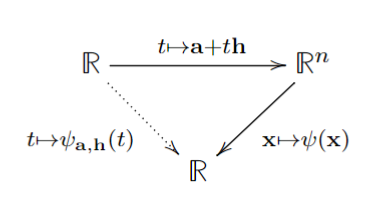
\includegraphics[width=0.3\linewidth]{image-1.png}
\end{figure}\\
Далее, для функции от одной переменной, значение её производной это есть значение дифференциала вычисленного в этой же точке. Тогда по теореме о композиции,
$$
\psi'_{\m{a},\m{h}}(t) = (\mathrm{d}\psi)_t = (\mathrm{d}f)_{\m{a}+t\m{h}} \cdot (\mathrm{d}\gamma)_t,
$$
где 
$$
\gamma(t): = \m{a}+t\m{h} = \begin{pmatrix}
a_1 + th_1 \\ \vdots \\ a_n + t h_n
\end{pmatrix}
$$
Тогда её матрица Якоби (=дифференциал) имеет вид
$$
\mathrm{d}\gamma = \begin{pmatrix}
\dot\gamma_1(t) \\ \vdots \\ \dot \gamma_n(t)
\end{pmatrix} = \begin{pmatrix}
h_1 \\ \vdots\\ h_n
\end{pmatrix} = \m{h},
$$
здесь $\gamma_1(t) = a_1 + th_1,\ldots, \gamma_n(t) = a_n+th_n.$
Тогда, получаем
$$\begin{aligned}
\psi'_{\m{a},\m{h}}(t) & = (\mathrm{d}\psi)_t = (\mathrm{d}f)_{\m{a}+t\m{h}} \cdot (\mathrm{d}\gamma)_t \\
&= (\mathrm{d}f)_{\m{a}+t\m{h}} \m{h} \\
&= \left.\frac{\partial f}{ \partial x_1}\right|_{\m{a} + t \m{h}} \cdot h_1 + \cdots + \left.\frac{\partial f}{ \partial x_n}\right|_{\m{a} + t \m{h}} \cdot h_n
\end{aligned}$$\qed

\subsection{Пусть $f: \mathbb{R}^{n} \rightarrow \mathbb{R}$ есть $m+1$ раз дифференцируемая функция в окрестности точки $\mathbf{a} \in \mathbb{R}^{n}$, то для всех $\mathbf{h}$ из окрестности точки $\mathbf{0}_{n}$ верно
$
f(\mathbf{a}+\mathbf{h})=f(\mathbf{a})+(\mathrm{d} f)_{\mathbf{a}} \mathbf{h}+\frac{1}{2 !}\left(\mathrm{d}^{2} f\right)_{\mathbf{a}} \mathbf{h}+\cdots+\frac{1}{m !}\left(\mathbf{d}^{m} f\right)_{\mathbf{a}} \mathbf{h}+\frac{1}{(m+1) !}\left(\mathbf{d}^{m+1} f\right)_{\mathbf{a}+\theta \mathbf{h}} \mathbf{h},
$
где $0<\theta<1$ и она зависит от $\mathbf{a}, \mathbf{h}$ и $m$}
Пусть $\varphi_{\m{a},\m{h}}(t): = f(\m{a}+t \m{h})$, $t \in [0,1]$, тогда она $m+1$ раз дифференцируема и 
$$
\varphi^{k}(t) = (\mathrm{d}^k_{\m{a}+t\m{h}}f)(\m{h}).
$$

Тогда её полином Тэйлора с остаточным мономом в форме Лагранже имеет вид
$$
\varphi(t) = \varphi(0) + \frac{\varphi'(0)}{1!}t + \frac{\varphi''(0)}{2!}t^2 + \cdots + \frac{\varphi^{(m)}(0)}{m!}t^m + \frac{\varphi^{(m+1)}(\theta)}{(m+1)!}t^{m+1}
$$
где $0 < \theta < t.$

Тогда, используя равенство 
$$
\varphi_{\m{a},\m{h}}^{k}(t) = (\mathrm{d}^k_{\m{a}+t\m{h}}f)(\m{h}), \qquad 1 \le k \le m+1.
$$
получаем
$$\begin{aligned}
\varphi(0) &=& f(\m{a}), \\
\varphi^{(k)}(0) &=& (\mathrm{d}^k_{\m{a}}f)(\m{h}), \qquad 1 \le k \le m,\\
\varphi^{(m+1)}(\theta) &=&(\mathrm{d}^k_{\m{a}+\theta \m{h}}f)(\m{h}).
\end{aligned}$$

Тогда мы можем записать
$$
\varphi(t) = f(\m{a}) + \sum_{k=1}^m \frac{(\mathrm{d}^k_{\m{a}}f)(\m{h})}{k!}t^k + \frac{( \mathrm{d}^k_{\m{a}+\theta \m{h}}f)(\m{h}) }{(m+1)!}t^{m+1},
$$
так как $\varphi(1) = f(\m{a}+\m{h})$, то подставляя $t=1$ в последней сумме мы получаем требуемое\qed
\label{2.3}


\subsection{Докажите, что подпространство $K$ в метрическом пространстве $(E, d)$ — компакт тогда и только тогда, когда из любого его покрытия множествами, открытыми в $E$, можно выделить конечное подпокрытие этими же множествами}
(1) Пусть $(K,d|_K)$ — компактное подпространство в $(E,d)$, и пусть $\{ \mathscr{U}_\alpha \}_{\alpha \in A}$ — его покрытие, т.е. $K = \displaystyle\bigcup_{\alpha \in A} \mathscr{U}_\alpha$, где все $\mathscr{U}_\alpha \subseteq K$ открыты в $K$, но тогда для каждого $\alpha \in A$ существует открытое множество $\widetilde{\mathscr{U}}_\alpha$ в $E$ такое, что $\widetilde{\mathscr{U}_\alpha} = \mathscr{U}_\alpha \cap K$

Тогда $K \subseteq \displaystyle\bigcup_{\alpha \in A} \widetilde{\mathscr{U}}_\alpha$. Так как $K$ — компакт, то можно найти конечное число множеств, скажем, $\mathscr{U}_1, \ldots, \mathscr{U}_n$, таких, что $K = \displaystyle\bigcup_{i=1}^n\mathscr{U}_i$, но тогда $K \subseteq \displaystyle\bigcup_{i=1}^n \widetilde{\mathscr{U}}_i$

(2) Пусть для любого покрытия $\{\widetilde{\mathscr{U}}_\alpha\}_{\alpha \in A}$ множества $K$ открытыми множествами из $E$ можно всегда найти конечное подпокрытие, скажем, $K \subseteq \displaystyle\bigcup_{i=1}^n \widetilde{\mathscr{U}}_i$, но тогда 
$$
K = K \cap \displaystyle\bigcup_{i=1}^n \widetilde{\mathscr{U}}_i= \displaystyle\bigcup_{i=1}^n \mathscr{U}_i
$$
при этом каждое $\mathscr{U}_\alpha : = \widetilde{\mathscr{U}}_\alpha \cap K$ — открыто в $K$\qed

\subsection{Докажите, что любое метрическое пространство удовлетворяет аксиоме отделимости Хаусдорфа; для любых двух различных точек найдутся их непересекающиеся окрестности}
Пусть $(E,d)$ — метрическое пространство, и пусть $x_1,x_2 \in E$ — две его различные точки. Нужно показать, что найдутся два открытых множества $\mathscr{U}_1, \mathscr{U}_2 \subset E$ такие, что $x_1\in \mathscr{U}_1$, $x_2\in \mathscr{U}_2$ и $\mathscr{U}_1\cap \mathscr{U}_2 = \varnothing$

Пусть $y \in B(x_1,r_1) \cap B(x_2,r_2)$, тогда $d(x_1,y)<r_1$ и $d(x_2,y)<r_2$. По неравенству треугольника, получаем
$$
d(x_1,x_2) \le d(x_1,y) + d(x_2,y)< r_1 +r_2
$$

Это означает, что $B(x_1,r_1) \cap B(x_2,r_2) \ne \varnothing$, если и только если $r_1+r_2 > d(x_1,x_2)$, а если $r_1+r_2 \le d(x_1,x_2)$, то $B(x_1,r_1) \cap B(x_2,r_2) = \varnothing$

Таким образом, для данных двух различных точек $x_1,x_2$ полагаем $\mathscr{U}_1: = B(x_1,r_1)$,\\
$\mathscr{U}_2:=B(x_2,r_2)$ и требуем, чтобы $r_1+r_2 \le d(x_1,x_2)$\qed
\label{2.5}

\subsection{Докажите, что в любом метрическом пространстве $(E, d)$ точка — замкнутое множество}
Пусть $y \in \overline{\{x\}}$ тогда для любого $r>0$, $B(y,r) \cap \{x\} \ne \varnothing$, т. е. для любого $r >0$ $x \in B(y,r)$, учитывая выполнения аксиомы отделимости в метрических пространствах получаем, что такое возможно, только если $x =y$\qed


\subsection{Докажите, что в метрическом пространстве ($E, d$) любой компакт обладает следующими свойствами:\\
(a) Компакт — ограниченное множество, т.е., найдётся такой шар $B(a, r) \subseteq E$, что $K \subseteq B(a, r)$;\\
(b) Компакт — замкнутое множество, т.е., он содержит все свои точки прикосновения ($\bar{K}=K)$;\\
(c) Замкнутое подмножество компакта самое является компактом}
Пусть $(E,d)$ — метрическое пространство, $K$ — компакт в $E$.
\label{2.7}

(1)  Согласно Аксиоме Выбора, мы можем взять точку $x\in K$. Рассмотрим бесконечную последовательность шаров $(B(x,n))_{n=1}^\infty$ в $K$, очевидно, что это — покрытие для $K$, и более того $E = \cup_{n \ge 1} B(x,n)$. Так как $K$ — компакт, то из этого покрытия можно выбрать конечное подпокрытие, скажем, $\{B(x,r)\}_{r=t}^N$, такое, что $K \subseteq \cup_{t=1}^N B(x,r)$. Так как $B(x,p) \subseteq B(x,q)$ при $p<q$, то $\cup_{t=1}^N B(x,r) = B(x,N)$, что и показывает ограниченность $K$\\[2mm]

(2) Ясно, что $K \subseteq \cup_{x \in K} B(x,r_x)$, для каких-то $r_x >0$. Так как $K$ — компакт, то можно найти конечное множество точек $\{x_1,\ldots, x_n\}$ такое, что $K \subseteq \cup_{i=1}^n B(x_i, r_i)$, где $r_i = r_{x_i}$, $1\le i \le n$

Пусть $y\in \overline{K}$, тогда для любого шара $B(y,r)$ имеем $B(y,r ) \cap K  \ne \varnothing$, и пусть $y\notin K$. Но тогда по лемме \ref{2.5} для каждого $1\le i \le n$ найдутся такие $\varepsilon_i>0$, что $B(y, \varepsilon_i) \cap B(x_i, r_i) = \varnothing$, тогда, полагая $\varepsilon: = \min \{\varepsilon_1, \ldots, \varepsilon_n\}$, получаем, что
$$
B(y, \varepsilon) \cap K \subseteq B(y, \varepsilon) \cap \bigcup_{i=1}^n B(x_i,r_i) = \varnothing,
$$
т.е. мы нашли окрестность $B(y, \varepsilon)$ точки $y$, которая не пересекается с $K$, что означает, что $y \notin \overline{K}$. Поэтому если $y\in \overline{K}$, то $y \in K$, т. е. $\overline{K} = K$\\[2mm]

(3) Пусть $F \subseteq K$ — замкнутое подмножество в $K$, и пусть $\{\mathscr{U}_\alpha\}_{\alpha \in A}$ — покрытие $F$ открытыми множествами из $E$, т. е. $F \subseteq \cup_{\alpha \in A} \mathscr{U}_\alpha$\\[2mm]

Тогда имеем
$$
K \subseteq F \cup (E \setminus F) \subseteq \bigcup_{\alpha \in A} \mathscr{U}_\alpha \cup (E \setminus F),
$$
т. е. мы получили покрытие для $K$, но так как $K$ — компакт, то можно найти такие, скажем, $\mathscr{U}_1, \ldots, \mathscr{U}_n$, что 
$$
K \subseteq \mathscr{U}_1 \cup \cdots \cup \mathscr{U}_n \cup (E \setminus F),
$$
но тогда 
$$
F \subseteq \mathscr{U}_1 \cup \cdots \cup \mathscr{U}_n,
$$
что означает компактность $F$\qed

\subsection{Докажите, что если $f:E\to E'$ — непрерывное отображение между метрическими пространствами, тогда если $X$ — компактно, то $f(X)$ — компактно}
Пусть $\{\mathscr{U}'_\alpha\}_{\alpha \in A}$ — покрытие $f(E)$ открытыми в $E'$ множествами, тогда $\{f^{-1}(\mathscr{U}'_\alpha)\}_{\alpha \in A}$ — покрытие $E$, и так как $f$ — непрерывно, тогда это покрытие открытыми множествами в $E.$ Так как $X$ — компактно, то можно найти конечное подпокрытие, скажем, $\{f^{-1}(\mathscr{U}'_i)\}_{i=1}^n$, но тогда $\{\mathscr{U}_i\}_{i=1}^n$ — покрытие для $f(X)$, что и показывает компактность $f(X)$\qed
\label{2.8}


\subsection{Докажите, что параллелепипед $\mathcal{P}$ — компакт в $\mathbb{R}^{n}$, где рассматривается евклидова метрика}
\textbf{(Прямоугольным) параллелепипедом в $\mathbb{R^n}$} будем называть множество 
$$
\mathcal{P}: = [a_1, b_1] \times \cdots \times [a_n, b_n]
$$
Доказывать будем от противного. Допустим, что существует такое покрытие $\{\mathscr{U}_\alpha\}_{\alpha \in A}$ открытыми множествами из $\mathbb{R}^n$ для параллелепипеда $\mathcal{P}$, что из него нельзя выбрать конечное подпокрытие. 
\label{2.9}

Итак, пусть $\mathcal{P} \subseteq \bigcup_{\alpha \in A} \mathscr{U}_\alpha$ и из этого покрытия нельзя выбрать конечное подпокрытие которое бы покрыло $\mathcal{P}$. Разобьём каждый отрезок $[a_k, b_k]$ пополам **т.е.,** представим его так
$$
[a_k, b_k] = \left[ a_k, \frac{a_k+b_k}{2} \right] \cup \left[\frac{a_k +b_k}{2}, b_k \right] \qquad 1 \le k \le n,
$$
тогда $\mathcal{P}$ разобьётся на $2^n$ параллелепипедов. По условию, $\mathcal{P}$ нельзя покрыть конечным числом множеств из $\{ \mathscr{U}_\alpha\}_{\alpha \in A}$, тогда найдётся хотя бы один из полученных параллелепипедов, обозначим его через $\mathcal{P}_1$, который тоже нельзя покрыть конечным числом множеств из покрытия $\{ \mathscr{U}_\alpha\}_{\alpha \in A}$.

Разобьём теперь параллелепипед $\mathcal{P}_1$ аналогичным образом на $2^n$ параллелепипедов. Так как $\mathcal{P}_1$ нельзя покрыть конечным числом множеств из покрытия $\{ \mathscr{U}_\alpha\}_{\alpha \in A}$, то найдётся хотя бы один, скажем $\mathcal{P}_2$, из только что полученных, который тоже нельзя покрыть конечным числом множеств. Будем повторять эту процедуру каждый раз. В результате мы получаем бесконечную цепь вложенных друг в друга параллелепипедов 
$$
\mathcal{P} \supsetneq \mathcal{P}_1 \supsetneq \mathcal{P}_2 \supsetneq \ldots
$$
каждый из которых нельзя покрыть конечным числом элементов множества $\{\mathscr{U}_\alpha\}_{\alpha \in A}$, и где каждый из них описывается следующим образом
$$
\mathcal{P}_i = \left[a_i^{(1)}, b_i^{(1)} \right] \times \cdots \times \left[a_i^{(n)}, b_i^{(n)} \right], \qquad i \ge 1,
$$
при этом, по построению, получаем $n$ систем вложенных друг в друга отрезков
\begin{align*}
& \left[ a_1^{(1)}, b_1^{(1)} \right] \supseteq \left[ a_2^{(1)}, b_2^{(1)} \right] \supseteq \left[ a_3^{(1)}, b_3^{(1)} \right] \supseteq \ldots \\
& \left[ a_1^{(2)}, b_1^{(2)} \right] \supseteq \left[ a_2^{(2)}, b_2^{(2)} \right] \supseteq \left[ a_3^{(2)}, b_3^{(2)} \right] \supseteq \ldots 
\end{align*}
у которых длины строго уменьшаются (каждый из отрезков по длине в два раза меньше чем его соседний слева отрезок). Тогда по Лемме о вложенных отрезках, для каждой из этих $n$ систем есть своя общая точка, $c_i \in \bigcap_{k \ge 1} [ a_k^{(i)}, b_k^{(i)} ] $, которая есть предельная для последовательности их концов; 

$$
\begin{matrix}
a_1^{(1)} & a_2^{(1)} & a_3^{(1)}& \ldots  & \to & c_1 & \leftarrow & \ldots & b_3^{(1)} & b_2^{(1)}  \\
a_1^{(2)} & a_2^{(2)} & a_3^{(2)}& \ldots  & \to & c_2 & \leftarrow & \ldots & b_3^{(1)} & b_2^{(1)}  \\
\vdots & \vdots &\vdots & \ddots && \vdots && && \\
a_1^{(n)} & a_2^{(n)} & a_3^{(n)}& \ldots  & \to & c_n & \leftarrow & \ldots & b_3^{(1)} & b_2^{(1)}  
\end{matrix}
$$

тогда для любого $\varepsilon >0$ и для каждого $1\le p \le n$, найдётся такой номер $M_p$, что при $m \ge M_p$ все $a_m^{(p)}, b_m^{(p)} \in (c_p - \varepsilon, c_p + \varepsilon)$. Пусть $M: = \max_{1 \le p \le n}\{M_p\}$, тогда при $m > M$ все $a_m^{(p)}, b_m^{(p)} \in (c_p - \varepsilon, c_p + \varepsilon)$ при любом $1\le p \le n.$

Рассмотрим теперь параллелепипед

$$
\mathcal{P}_\varepsilon(\m{c}):= [c_1 - \varepsilon, c_1 + \varepsilon] \times \cdots \times [c_n - \varepsilon, c_n + \varepsilon]
$$
где $\m{c}: = (c_1,\ldots, c_n)$. Тогда, для всех $m>M$, получаем что все параллелепипеды $\mathcal{P}_m \subset \mathcal{P}_\varepsilon(\m{c})$.

С другой стороны, 

$$
\m{c} = (c_1,\ldots, c_n) \in \bigcap_{i \ge 1} \mathcal{P}_i \subset \mathcal{P} \subseteq \bigcup_{\alpha \in A} \mathscr{U}_\alpha
$$
тогда найдётся хотя бы одно $\mathscr{U}_\alpha$ содержащее это точку $\m{c}$, так как $\mathscr{U}_\alpha$ открыто, то найдётся шар $B(c, r)$ такой, что $B(\m{c}, r) \subseteq \mathscr{U}_\alpha$.

Пусть теперь $0 < \varepsilon < \dfrac{r}{\sqrt{n}}$, тогда получаем, что для каждого $m>M$

$$
\mathcal{P}_m \subseteq \mathcal{P}_\varepsilon(\m{c}) \subseteq B(\m{c}, r) \subseteq \mathscr{U}_\alpha.
$$

Но это означает что, каждый из $\mathcal{P}_m$ при $m >M$ можно покрыть всего одним элементом $\mathscr{U}_\alpha$, что противоречит выбору таких параллелепипедов, т.е., первоначальный параллелепипед можно тогда покрыть конечным числом элементов множества $\{\mathscr{U}_\alpha\}$, что означает его компактность\qed

\subsection{Докажите критерий компактности в $\mathbb{R}^{n}$; множество $K \subseteq \mathbb{R}^{n}$ компактно тогда и только тогда когда оно замкнуто и ограничено}
(1) Согласно свойствам компакта из \ref{2.7} мы получаем необходимость
\label{2.10}

(2) Если $K \subseteq \mathbb{R}^n$ ограниченно и замкнуто, то это значит, что оно содержится в некотором шаре, скажем, $B(\m{x}, r)$ который содержится целиком внутри параллелепипеда
$$
\mathcal{P} = [x_1- r,x_1+r] \times \cdots \times [x_n-r, x_n+r]
$$
где $\m{x} = (x_1, \ldots, x_n)$. Так как $K$ — замкнуто, то из предложения из \ref{2.9} и свойств компакта \ref{2.7} вытекает утверждение\qed


\subsection{Докажите, что на компактном множестве всякая непрерывная функция ограничена и достигает наибольшего и наименьшего значений}
Другими словами, если $f:K \to \mathbb{R}$ — непрерывная функция, $K$ — компактно, то найдутся такие $a,b \in X$, что $f(a) \le f(x) \le f(b)$ для любого $x \in X$\\

Согласно п.\ref{2.8} $f(K)$ — компактно в $\mathbb{R}$, тогда согласно критерию компактности в $\mathbb{R}^n$ (п. \ref{2.10}) оно ограничено. Тогда согласно принципу полноты Вейерштрасса существуют $m:=\inf f(X)$, $M:= \sup f(X)$

Но, согласно критерию компактности в $\mathbb{R}^n$ (п.\ref{2.10}) $f(X)$ также и замкнуто, тогда $m,M \in f(X)$, откуда и следует существование таких точек $a,b\in X$, что $f(a) \le f(x) \le f(b)$ при всех $x\in X$\qed


\subsection{Пусть $f: \mathbb{R}^{n} \rightarrow \mathbb{R}$ есть $m$ раз дифференцируема функция в окрестности точки а и все её частные производные непрерывны в этой точке, тогда $f(\mathbf{a}+\mathbf{h})=f(\mathbf{a})+(\mathrm{d} f)_{\mathbf{a}} \mathbf{h}+\frac{1}{2 !}\left(\mathrm{d}^{2} f\right)_{\mathbf{a}} \mathbf{h}+\cdots+\frac{1}{m !}\left(\mathbf{d}^{m} f\right)_{\mathbf{a}} \mathbf{h}+o\left(\|\mathbf{h}\|^{m}\right),\mathbf{h} \rightarrow \mathbf{0}_{n}$}
По теореме \ref{2.3}, 
$$
f(\m{a} + \m{h}) = f(\m{a}) + (\mathrm{d}f)_\m{a} \m{h} + \frac{1}{2!} (\mathrm{d}^2f)_\m{a}\m{h} + \cdots + \frac{1}{(m-1)!} (\m{d}^{m-1}f)_\m{a}\m{h} + \frac{1}{m!} (\m{d}^{m}f)_{\m{a}+ \theta \m{h}}\m{h},
$$
рассмотрим последний моном (самый правый) этого полинома, имеем
$$
(\m{d}^{m}f)_{\m{a}+ \theta \m{h}}(\m{h})= (\m{d}^{m}f)_{\m{a}}(\m{h}) +  \Bigl( (\m{d}^{m}f)_{\m{a}+ \theta \m{h}}(\m{h}) - (\m{d}^{m}f)_{\m{a}} (\m{h}) \Bigr).
$$

Согласно теореме \ref{2.1}, 
$$
(\mathrm{d}^mf)_{\m{b}}(\m{h}) = \sum_{p_1 + \ldots + p_n = m} \dfrac{m!}{p_1! \cdots p_n!} \left.\frac{\partial^m f}{\partial x_1^{p_1} \cdots \partial x_n^{p_n}}\right|_{\m{b}} \cdot h_1^{p_1}\cdots h_n^{p_n},
$$
тогда, получаем
$$\begin{aligned}
(\m{d}^{m}f)_{\m{a}+ \theta \m{h}}(\m{h}) &= (\m{d}^{m}f)_{\m{a}}(\m{h}) +  \Bigl( (\m{d}^{m}f)_{\m{a}+ \theta \m{h}}(\m{h}) - (\m{d}^{m}f)_{\m{a}} (\m{h}) \Bigr) \\
&= (\m{d}^{m}f)_{\m{a}}(\m{h}) + \sum_{p_1 + \ldots + p_n = m} \dfrac{m!}{p_1! \cdots p_n!}\left( \left.\frac{\partial^m f}{\partial x_1^{p_1} \cdots \partial x_n^{p_n}}\right|_{\m{a}+\theta \m{h}} - \left.\frac{\partial^m f}{\partial x_1^{p_1} \cdots \partial x_n^{p_n}}\right|_{\m{a}} \right)\cdot h_1^{p_1}\cdots h_n^{p_n} \\
&= (\m{d}^{m}f)_{\m{a}}(\m{h})\\
&+ \|h \|^m \sum_{p_1 + \ldots + p_n = m} \dfrac{m!}{p_1! \cdots p_n!}\left( \left.\frac{\partial^m f}{\partial x_1^{p_1} \cdots \partial x_n^{p_n}}\right|_{\m{a}+\theta \m{h}} - \left.\frac{\partial^m f}{\partial x_1^{p_1} \cdots \partial x_n^{p_n}}\right|_{\m{a}} \right) \frac{h_1^{p_1}}{\|h\|^{p_1}} \cdots \frac{h_n^{p_n}}{\|h\|^{p_n}}.
\end{aligned}$$

Так как $\| h \|: = \sqrt{h_1^2 + \cdots + h_n^2}$, то 
$$
\frac{h_1^{p_1}}{\| \m{h}\|^{p_1}}, \ldots, \frac{h_1^{p_1}}{\| \m{h}\|^{p_1}} \le 1 
$$
далее, так как все частные производные непрерывны в точке $\m{a}$, то по критерию непрерывности,
$$
\lim_{\m{h} \to \m{0}_n} \left( \left.\frac{\partial^m f}{\partial x_1^{p_1} \cdots \partial x_n^{p_n}}\right|_{\m{a}+\theta \m{h}} - \left.\frac{\partial^m f}{\partial x_1^{p_1} \cdots \partial x_n^{p_n}}\right|_{\m{a}} \right) = 0, 
$$
при каждом разбиении $m = p_1 + \cdots + p_n$, таким образом, 
$$
\lim_{\m{h} \to \m{0}_n} \sum_{p_1 + \ldots + p_n = m} \dfrac{m!}{p_1! \cdots p_n!}\left( \left.\frac{\partial^m f}{\partial x_1^{p_1} \cdots \partial x_n^{p_n}}\right|_{\m{a}+\theta \m{h}} - \left.\frac{\partial^m f}{\partial x_1^{p_1} \cdots \partial x_n^{p_n}}\right|_{\m{a}} \right) = 0,
$$
а это и означает, что 
$$
(\m{d}^{m}f)_{\m{a}+ \theta \m{h}}(\m{h}) = (\m{d}^{m}f)_{\m{a}}(\m{h}) + \omega(\m{h}) \|h\|^m, \quad \m{h} \to \m{0}_n,
$$
где $\lim\limits_{\m{h} \to \m{0}_n} \omega(\m{h}) = \m{0}_n$, \textbf{т.е.,}
$$
(\m{d}^{m}f)_{\m{a}+ \theta \m{h}}(\m{h}) = (\m{d}^{m}f)_{\m{a}}(\m{h}) + o(\|h\|^m), \quad \m{h} \to \m{0}_n,
$$
но тогда
$$\begin{aligned}
f(\m{a} + \m{h}) &= f(\m{a}) + (\mathrm{d}f)_\m{a} \m{h} + \frac{1}{2!} (\mathrm{d}^2f)_\m{a}\m{h} + \cdots + \frac{1}{(m-1)!} (\m{d}^{m-1}f)_\m{a}\m{h} + \frac{1}{m!} (\m{d}^{m}f)_{\m{a}+ \theta \m{h}}\m{h} \\
&=f(\m{a}) + (\mathrm{d}f)_\m{a} \m{h} + \frac{1}{2!} (\mathrm{d}^2f)_\m{a}\m{h} + \cdots + \frac{1}{(m-1)!} (\m{d}^{m-1}f)_\m{a}\m{h} + \frac{1}{m!}\left( (\mathrm{d}^mf)_\m{a} (\m{h}) + o(\|\m{h}\|^m) \right) \\
&=f(\m{a}) + (\mathrm{d}f)_\m{a} \m{h} + \frac{1}{2!} (\mathrm{d}^2f)_\m{a}\m{h} + \cdots + \frac{1}{m!} (\m{d}^mf)_\m{a}\m{h} + o(\| \m{h} \|^m), \qquad \m{h} \to \m{0}_n
\end{aligned}$$\qed
\label{2.12}

\subsection{Если функция $f: \mathbb{R}^{n} \rightarrow \mathbb{R}$ — дважды дифференцируема в точке а, то
$f(\mathbf{a}+\mathbf{h})=f(\mathbf{a})+\nabla_{\mathbf{a}}(f)(\mathbf{h})+\frac{1}{2} \mathbf{h}^{\top} \mathbf{H}_{\mathbf{a}}(f) \mathbf{h}+o\left(\|\mathbf{h}\|^{2}\right), \mathbf{h} \rightarrow \mathbf{0}_{n}$}

Согласно п. \ref{2.12} , 
$$
f(\m{a} + \m{h}) = f(\m{a}) + (\mathrm{d}f)_\m{a} \m{h} + \frac{1}{2} (\mathrm{d}^2f)_\m{a}\m{h} + o(\| \m{h} \|^2), \qquad \m{h} \to \m{0}_n,
$$
но $(\mathrm{d}f)_\m{a} \m{h} = \nabla_\m{a}(f)(\m{h})$. Далее, по теореме \ref{2.1},
$$\begin{aligned}
(\mathrm{d}^kf)_\m{a}(\m{h})  &= \left.\left(\frac{\partial}{\partial x_1} h_1 + \cdots + \frac{\partial }{\partial x_n}h_n \right)^2\right|_{\m{a}} \cdot f \\
&= \sum_{i=1}^n \left.\dfrac{\partial^2 f}{\partial x_i^2} \right|_\m{a} h_i^2 + 2 \sum_{1\le i < j \le n}  \left.\dfrac{\partial^2 f}{\partial x_i \partial x_j} \right|_{\m{a}} h_ih_j,
\end{aligned}$$
где $\m{h} = (h_1, \ldots, h_n)^n$, но последнее выражение можно записать в матричном виде следующим образом
$$
(h_1, \ldots, h_n)^\top \begin{pmatrix}
\left.\dfrac{\partial^2 f}{\partial x_1^2}\right|_{\m{a}} & \left.\dfrac{\partial^2 f}{\partial x_1 \partial x_2}\right|_{\m{a}} &\ldots & \left.\dfrac{\partial^2 f}{\partial x_1 \partial x_n}\right|_{\m{a}} \\
\left.\dfrac{\partial^2 f}{\partial x_2 \partial x_1}\right|_{\m{a}} & \left.\dfrac{\partial^2 f}{\partial x_2^2}\right|_{\m{a}} & \ldots & \left.\dfrac{\partial^2 f}{\partial x_2 \partial x_n}\right|_{\m{a}} \\
\vdots & \vdots & \ddots & \vdots \\
\left.\dfrac{\partial^2 f}{\partial x_n \partial x_1}\right|_{\m{a}} & \left.\dfrac{\partial^2 f}{\partial x_n \partial x_2}\right|_{\m{a}} & \ldots &\left.\dfrac{\partial^2 f}{ \partial x_n^2}\right|_{\m{a}}
\end{pmatrix} \begin{pmatrix}
h_1 \\ \vdots \\ h_n
\end{pmatrix}  =  \m{h}^\top \m{H}_\m{a}(f) \m{h} ,
$$
и так как матрица симметрична, доказано требуемое\qed
\label{2.13}

\subsection{Докажите необходимое условие экстремума}
\textbf{Условие.} Если $\m{a} = (a_1,\ldots, a_n) \in \mathbb{R}^n$ — точка экстремума функции $f:\mathbb{R}^n \to \mathbb{R}$, тогда, если все частные производные $f'_{x_i}$, $1\le i \le n$ существуют в какой-то окрестности $\mathscr{U}(\m{a})$ точки $\m{a}$, то $(\mathrm{d}f)_\m{a}(\m{h}) = 0$ для любого $\m{h} \in \mathscr{U}(\m{a}),$ или
$$
\left.\frac{\partial f}{\partial x_1}\right|_\m{a} = \ldots = \left.\frac{\partial f}{\partial x_1}\right|_\m{a} = 0.   
$$

\textbf{Доказательство.} Рассмотрим $k$ функций $\varphi_k(t): = f(a_1,\ldots, a_{k-1}, t, a_{k+1}, \ldots, a_n)$, $1 \le k \le n$, где от каждого $t$ мы требуем, чтобы соответствующая точка лежала в окрестности $\mathscr{U}(\m{a})$

Пусть $\m{a}$ — точка максимума, тогда, в частности, $f(a_1, \ldots, t, \ldots) \le f(\m{a})$ для любого $t$, т.е. $\varphi_k(t) \le f(\m{a})$ при каждом $1 \le k \le n$

Другими словами, $a_k$ — точка максимума для $\varphi_k(t)$. Тогда по теореме Ферма, $\varphi'_k(a_k) = 0$, но $\varphi'_k(a_k) = f'_{x_k}(\m{a}) = 0$ для каждого $1 \le k \le n$\qed

\subsection{Докажите необходимое условие условного экстремума}
\textbf{Условие.} Пусть $f, \varphi_1,\ldots, \varphi_m: \mathbb{R}^{n+m} \to \mathbb{R}$ являются непрерывно дифференцируемыми фукнциями в окрестности $\mathscr{W}$ точки $\m{a}$, и пусть 
$$
\mathrm{rk} \begin{pmatrix}
\dfrac{\partial \varphi_1}{\partial x_1} (\m{x}) & \ldots & \dfrac{\partial \varphi_1}{\partial x_{n+m}} (\m{x}) \\
\vdots & \ddots & \vdots \\
\dfrac{\partial \varphi_m}{\partial x_1} (\m{x}) & \ldots & \dfrac{\partial \varphi_m}{\partial x_{n+m}} (\m{x})
\end{pmatrix} = m
$$
для всех $\m{x}\in \mathscr{W}$. Тогда, если $\m{a}$ — точка условного экстремума функции $f$ на множестве
$$
\Omega: = \{\m{x} \in \mathbb{R}^{n+m}\,:\, \varphi_1(\m{x}) =0, \ldots, \varphi_m(\m{x}) = 0\}
$$
то найдутся такие числа $\lambda_1,\ldots, \lambda_m \in \mathbb{R}$, что
$$
\nabla_\m{a} f = \lambda_1 \nabla_\m{a} \varphi_1 + \cdots +   \lambda_m \nabla_\m{a} \varphi_m
$$

\textbf{Доказательство.} Рассмотрим отображение
$$
\Phi: \mathbb{R}^{n+m} \to \mathbb{R}^{n+m}, \qquad \begin{pmatrix}
x_1 \\ \vdots \\ x_m \\ x_{m+1} \\ \vdots \\ x_{n+m}
\end{pmatrix} \mapsto \begin{pmatrix}
\varphi_1(x_1,\ldots, x_{n+m}) \\
\vdots \\
\varphi_m(x_1,\ldots, x_{n+m}) \\
x_{m+1} \\ \vdots \\x_{n+m}
\end{pmatrix}
$$
согласно условиям, оно непрерывно дифференцируемо в окрестности $\mathscr{W}$ точки $\m{a}$

Сделаем замену переменных
\begin{equation}\label{coordantes_u}
\begin{matrix}
u_1 & = & \varphi_1(x_1,\ldots, x_{n+m}) \\
\vdots & & \vdots\\
u_m & = & \varphi_m(x_1,\ldots, x_{n+m}) \\
u_{m+1} &=& x_{m+1} \\
\vdots && \vdots \\
u_{m+n} &=& x_{m+n}
\end{matrix}
\end{equation}

Если нужно, то, перенумеровав переменные, можно считать, что из условия о ранге матрицы вытекает
$$
\mathrm{det} \begin{pmatrix}
\dfrac{\partial \varphi_1}{\partial x_{1}}(\m{x}) &\ldots& \dfrac{\partial \varphi_1}{\partial x_{m}}(\m{x}) \\
\vdots & \ddots & \vdots \\
\dfrac{\partial \varphi_m}{\partial x_{1}}(\m{x}) &\ldots & \dfrac{\partial \varphi_m}{\partial x_{m}}(\m{x})
\end{pmatrix} \ne 0
$$

Тогда по теореме об обратном отображении (\ref{1.10}), $\Phi$ — локально обратима в окрестности $\mathscr{U} \subseteq \mathscr{W}$ точки $\m{a}.$ Это значит, что существуют такие непрерывно дифференцируемые функции $\psi_i: \mathscr{V} \to \mathbb{R}$, $1\le i \le n+m$, где $\mathscr{V}$ — окрестность точки $\Phi(\m{a})$, что мы получаем обратную замену координат к замене (\ref{coordantes_u}) 
$$
\begin{matrix}
x_1 & = & \psi_1(u_1,\ldots, u_{m}) \\
\vdots & & \vdots\\
x_{n+m} & = & \psi_{n+m}(u_1,\ldots, u_m)
\end{matrix}
$$\newpage
В итоге, мы получаем две коммутативные диаграммы
\begin{center}
    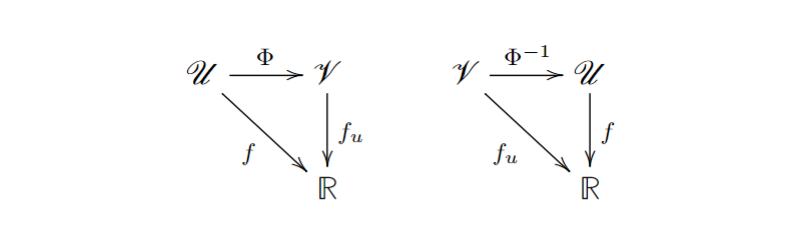
\includegraphics[width=0.5\linewidth]{image-4.png}
\end{center}
\textbf{т.е.,}
$$
f_u(u_1, \ldots, u_{n+m}) := f(\varphi_1(x_1,\ldots, x_{n+m}), \ldots, \varphi_m(x_1,\ldots, x_{n+m}), x_{m+1},\ldots, x_{m+n}),
$$
и
$$
f(x_1,\ldots, x_{n+m})= f_u(\psi_1(u_1,\ldots, \psi_m), \ldots, \psi_{n+m}(u_1,\ldots, u_m)).
$$

Тогда, если мы ограничимся рассмотрением точек на множестве $\Omega$, то во-первых, мы получаем, что 
$$
\Phi(\Omega) = \{(u_1,\ldots, u_{n+m}) \in \mathscr{U}\, : \, u_1=0,\ldots, u_m=0\},
$$
во-вторых мы получаем функцию уже от $n$ переменных $f_u(0,\ldots, 0, u_{m+1},\ldots, u_{m+n})$

Далее, из диаграммы
\begin{center}
    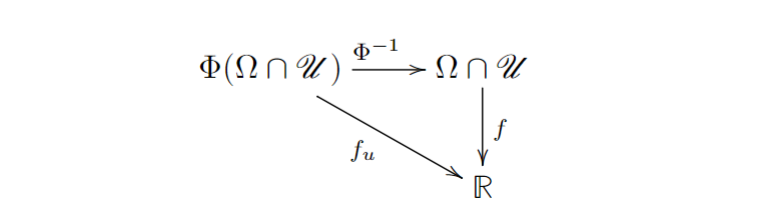
\includegraphics[width=0.5\linewidth]{image-5.png}
\end{center}
следует, что при $\m{y} \in \Phi(\Omega \cap \mathscr{U})$, отображение $\Phi^{-1}$ имеет вид
$$
\qquad \Phi^{-1} : \begin{pmatrix}
0\\
\vdots \\
0\\
u_{m+1} \\
\vdots \\
u_{m+n}
\end{pmatrix} \mapsto \begin{pmatrix}
0\\
\vdots \\
0\\
x_{m+1} \\
\vdots \\
x_{m+n}
\end{pmatrix},
$$
а так как $u_{m+1} = x_{m+1}, \ldots, u_{m+n} =x_{n+m}$, то
$$
f_u(0,\ldots, 0, u_{m+1},\ldots, u_{m+n}) = f(0,\ldots, 0, x_{m+1}, \ldots, x_{n+m}) \circ \Phi^{-1}.
$$

Но тогда $\Phi(\m{a})$ — точка экстремума функции $f_u(0,\ldots, 0, u_{m+1},\ldots, u_{m+n})$ и по необходимому признаку, мы получаем
$$
\dfrac{\partial f_u}{\partial{u_{m+1}}}(\Phi(\m{a})) = \cdots = \dfrac{\partial f_u}{\partial{u_{m+n}}}(\Phi(\m{a})) = 0.
$$

Это значит, что в точке $\Phi(\m{a})$ имеем
$$
(\mathrm{d}f_u)_{\Phi(\m{a})} = \begin{pmatrix}
\lambda_1 & \ldots & \lambda_m & 0 & \ldots & 0
\end{pmatrix}.
$$

Наконец, из диаграммы

\begin{center}
    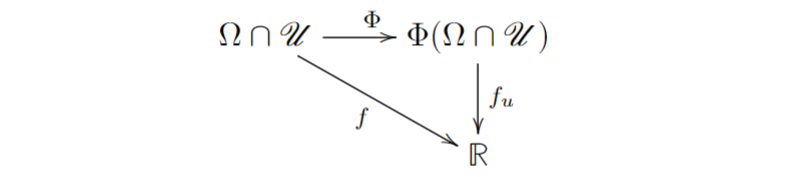
\includegraphics[width=0.5\linewidth]{image-6.png}
\end{center}

и из теоремы о композиции дифференциалов получаем
$$\begin{aligned}
(\mathrm{d}f)_\m{a} &= (\mathrm{d}f_u)_{\Phi(\m{a})} \cdot (\mathrm{d}\Phi)_{\m{a}} \\
&= \begin{pmatrix}
\lambda_1 & \ldots & \lambda_m & 0 & \ldots 0
\end{pmatrix} \begin{pmatrix}
\dfrac{\partial \varphi_1}{\partial x_1}(\m{a}) & \ldots & \dfrac{\partial \varphi_1}{\partial x_m}(\m{a}) & \dfrac{\partial \varphi_1}{\partial x_{m+1}}(\m{a}) & \ldots & \dfrac{\partial \varphi_1}{\partial x_{m+n}}(\m{a}) \\
\vdots & \ddots & \vdots & \vdots & \ddots & \vdots\\
\dfrac{\partial \varphi_m}{\partial x_1}(\m{a}) & \ldots & \dfrac{\partial \varphi_m}{\partial x_m}(\m{a}) & \dfrac{\partial \varphi_n}{\partial x_{m+1}}(\m{a}) & \ldots & \dfrac{\partial \varphi_m}{\partial x_{m+n}}(\m{a}) \\
0 & \ldots & 0 & 1 & \ldots &0 \\
\vdots & \ddots & \vdots & \vdots & \ddots & \vdots\\
0 & \ldots & 0 & 0 & \ldots & 1
\end{pmatrix} \\
&= \lambda_1 (\mathrm{d}\varphi_1)_{\m{a}} + \ldots + \lambda_m (\mathrm{d}\varphi_m)_{\m{a}}
\end{aligned}$$\qed

\subsection{Докажите критерий сходимости Коши для рядов и выведете необходимый признак сходимости ряда. Этот признак достаточен? Ответ обоснуйте}
\textbf{Формулировка.} Ряд $(x_n)_{n\ge 1}$ сходится, если и только если для любого $\varepsilon >0$ существует такой номер $N$, что при $n \ge N$, $p\ge 1$ имеет место неравенство
$$
|s_{n+p} -s_n| = |x_{n+1}+ \cdots + x_{n+p}| < \varepsilon
$$

\textbf{Доказательство.} Для ряда $(x_n)$ рассмотрим последовательность $(s_n)$ его частичных сумм, тогда согласно определению, $(x_n)$ сходится, если и только если $\lim\limits_{n \to \infty} s_n = s$, а тогда по критерию Коши $(s_n)$ — фундаментальная, т.е. мы получаем следующее: $(s_n)$ — сходится, если и только если для любого $\varepsilon >0$ существует такой номер $N$, что при всех $n,m \ge N$, $|s_m- s_n| < \varepsilon$

Без ограничения общности мы можем положить, что $m>n$, т.е. $m= n+p$, где $p \ge 1$, в результате получаем следующее: последовательность $(s_n)$ сходится, если и только если для любого $\varepsilon >0$ существует такой номер $N$, что для любого $n \ge N$, $p \ge 1$ имеет место
$$
|s_{n+p} - s_n| = |x_{n+1} + \cdots+  x_{n+p}| < \varepsilon
$$\qed

\textbf{Необходимый признак.} Если ряд $(x_n)$ сходится, то 
$$
\lim_{n \to \infty} x_n =0
$$

\textbf{Доказательство.} Достаточно воспользоваться критерием сходимости Коши в случае, когда $p=1$, мы тогда получим что для любого $\varepsilon >0$ существует такой номер $N$, что при всех $m \ge N$, имеет место неравенство $|s_{m+1} - s_m| < \varepsilon$, но это означает, что $\lim\limits_{m \to \infty} (s_{m+1} - s_m)=0$

С другой стороны, 
$$\begin{aligned}
s_{m+1} -s_m &=& x_1 + \cdots x_m + x_{m+1} \\
&& - x_1 - \cdots - x_m \\
&=& x_{m+1},
\end{aligned}$$
поэтому из сходимости ряда $(x_n)$ следует, что $\lim\limits_{m\to \infty }x_{m+1} = 0$, теперь полагая $m = n-1$ и принимая во внимание соглашение $s_0 :=0$, получаем необходимое\qed

Необходимое условие ни в коем случае не является достаточным. Например, гармонический ряд этому условию удовлетворяет, но он не сходится

\subsection{Докажите, что если ряды $\left(x_{n}\right)$ и $\left(x_{n}^{\prime}\right)$ сходятся и имеют суммы $s$ и $s^{\prime}$, соотвественно, то ряд ($x_{n}+x_{n}^{\prime}$) сходится к сумме $s+s^{\prime}$, а ряд ($\lambda x_{n}$) для любого $\lambda \in \mathbb{R}$ — к сумме $\lambda s$}
(1) Последовательность частичных сумм ряда $(x_n + x_n')$ имеет вид 
$$
(x_1 + \cdots + x_n + x_1' + \cdots +x_n')
$$
т.е. $(s_n + s_n')$, но тогда по арифметике предела для последовательностей получаем $\lim\limits_{n \to \infty} (s_n + s_n') = s+ s'$, что доказывает первое утверждение\\[2mm]

(2) Последовательность частичных сумм для ряда $(\lambda x_n)$ имеет вид $(\lambda x_1 + \cdots + \lambda x_n)$, т.е. $(\lambda s_n)$, опять воспользовавшись арифметикой предела для последовательностей, мы завершаем доказательство\qed
\label{2.17}
\subsection{Докажите, что если $\left(x_{n}\right)$ и $\left(x_{n}^{\prime}\right)$ почти похощие ряды, то оба они сходятся или расходятся}
Рассмотрим ряд $(x_n''): = (x_n - x_n')$, тогда почти все его элементы равны нулю, а это значит, что он сходится, т. е. мы имеем $ \lim\limits_{n \to \infty} s''_n = s''$
\label{2.18}

(1) Пусть ряд $(x_n')$ сходится, и пусть $\lim\limits_{n \to \infty}s_n' =s'$, тогда согласно предложению \ref{2.17}, ряд $(x_n'' + x_n')$ ряд тоже сходится к сумме $s''+s'$, но $x_n''+x_n' = x_n$, т. е. ряд $(x_n)$ сходится

(2) Пусть теперь ряд $(x_n')$ расходится, а ряд $(x_n)$ сходится. Опять рассмотрим ряд $(x_n''): = (x_n - x_n')$, у которого почти все элементы нулевые, а значит, он сходится, и мы опять положим $\lim\limits_{n \to \infty}s_n'' = s''.$ Рассмотрим ряд $(x_n - x_n'')$, исходя из п. \ref{2.17}, получаем, что этот ряд сходится, но $x_n - x_n'' = x_n'$, и мы тем самым пришли к тому, что ряд $(x_n')$ сходится, что противоречит предположению, следовательно, ряд $(x_n)$ не может быть сходящимся, т.е. из расходимости ряда $(x_n')$ следует расходимость ряда $(x_n)$\qed

\subsection{Докажите критерий сходимости положительного ряда}
\label{2.19}
\textbf{Формулировка.} Положительный ряд $(x_n)$ сходится тогда и только тогда, когда последовательность $(s_n)$ его частичных сумм ограничена\\[2mm]
\indent\textbf{Доказательство.} В таком случае последовательность $(s_n)$ его частичных сумм строго возрастает, тогда если последовательность $(s_n)$ ограничена, то по теореме Вейрштрасса она имеет предел, т.е. ряд сходится

С другой стороны, пусть ряд сходится, тогда $\lim\limits_{n\to \infty} s_n =s$, т.е. для любого $\varepsilon >0$ найдётся такой номер $N$, что при всех $n \ge N$, $s-\varepsilon < s_n < s+ \varepsilon$, но $(s_n)$ — возрастающая, значит все $s_i < s + \varepsilon$, т.е. последовательность $(s_n)$ ограничена\qed


\subsection{Пусть $\left(x_{n}\right),\left(x_{n}^{\prime}\right)$ — два положительных ряда, при этом $x_{n} \leq x_{n}^{\prime}$ почти для всех $n$. Если ряд $\left(x_{n}^{\prime}\right)$ сходится, то сходится и ряд $\left(x_{n}\right)$. Если же ряд $\left(x_{n}\right)$ расходится, то расходится и ряд $\left(x_{n}^{\prime}\right)$}
Если неравенства $x_n\le x_n'$ не выпонены для каких-то конечных значений $n$, скажем, $n = n_1,\ldots, n_\ell$, то рассмотрим ряды $(y_n)$, $(y_n')$, определённые следующим образом:
$$
y_n = \begin{cases}
x_n, & n \ne n_1,\ldots, n_\ell,\\
0, & n = n_1,\ldots, n_\ell,
\end{cases} \qquad  y'_n = \begin{cases}
x'_n, & n \ne n_1,\ldots, n_\ell,\\
0, & n = n_1,\ldots, n_\ell
\end{cases} 
$$
которые почти похожи на ряды $(x_n)$ и $(x_n')$ соответственно. Согласно п. \ref{2.18}, ряды $(y_n)$, $(y_n')$ имеют тот же характер сходимости, как и ряды $(x_n)$, $(x_n')$ соответственно. Поэтому исследование характера сходимости рядов $(x_n)$, $(x_n')$ сводится к исследованию характера рядов $(y_n)$, $(y_n')$. Это означает, что мы без ограничения общности можем считать, что неравенства $x_n \le x_n'$ выполняются для всех $n\ge 1$

(1) Пусть ряд $(x_n')$ сходится, тогда согласно критерию сходимости положительного ряда (п.\ref{2.19}), последовательность его частичных сумм $(s_n')$ ограничена, скажем, числом $\alpha$, т.е. $s'_n < \alpha$ для всех $n.$ С другой стороны, по условию, $x_n \le x_n'$, тогда в силу положительности рядов
$$
s_n = x_1 + \cdots + x_n \le x_1' + \cdots + x_n' = s_n' < \alpha
$$
для всех $n$, т.е. последовательность частичных сумм ряда $(x_n)$ ограничена, тогда по критерию \ref{2.19}, ряд $(x_n)$ сходится

(2) Пусть ряд $(x_n)$ расходится, тогда по критерию \ref{2.19}, последовательность $(s_n)$ неограничена. Так как последовательность $(s_n)$ возрастает, то неограниченность означает, что для любого числа $M \in \mathbb{N}$ найдётся такой номер $n\in \mathbb{N}$, что все $s_n, s_{n+1}, \ldots > M$. С другой стороны, как мы уже видели, $s_n' \ge s_n$, таким образом, для всех $m \ge n$ получаем $s'_m \ge s_m > M$, т.е. последовательность $(s_n')$ неограничена, а тогда по по критерию \ref{2.19}, ряд $(x_n')$ расходится\qed







\end{document}


